\documentclass[border=1pt]{standalone}
\usepackage[dvipsnames]{xcolor}
\usepackage{tikz}                       % Graphen und kommutative Diagramme
\usetikzlibrary{patterns}               % Um schraffierte Formen in der tikzpicture-Umgebung zu zeichnen.

\newcommand{\ul}[1]{\underline{\smash{#1}}}

\begin{document}
\centering
\begin{minipage}{.55\textwidth}
\resizebox{\textwidth}{!}{
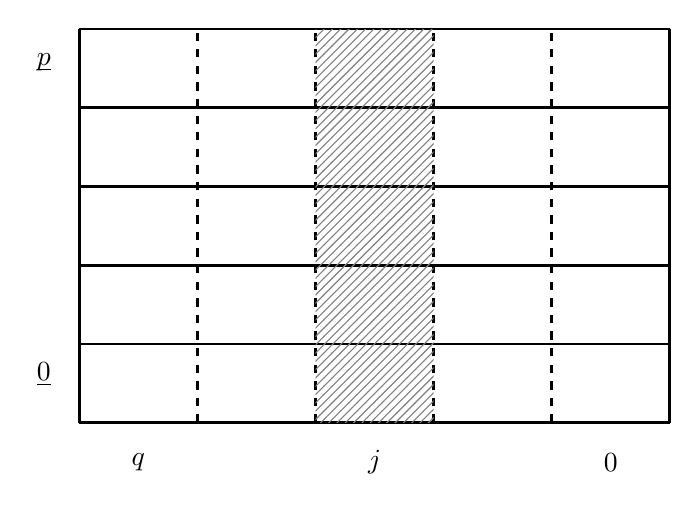
\begin{tikzpicture}[yscale=.8, xscale=1.2, x=1.25cm, y=1.25cm, line width=1pt]
    % Linien.
    \foreach \i in {0,...,5}
    {
        \draw[color=black] (0,\i) -- (5,\i);
    }
    \draw[color=black] (0,0) -- (0,5);
    \draw[color=black] (5,0) -- (5,5);
    \foreach \i in {1,...,4}
    {
        \draw[color=black, dashed] (\i,0) -- (\i,5);
    }
    
    % Beschriftung.
    \draw node at (-.3,4.5) {$\ul p$};
    \draw node at (-.3,0.5) {$\ul 0$};
    
    \draw node at (0.5,-.5) {$q$};
    \draw node at (2.5,-.5) {$j$};
    \draw node at (4.5,-.5) {$0$};
    
    \fill[pattern=north east lines, pattern color=gray] (2,0) -- (3,0) -- (3,5) -- (2,5) -- cycle;
\end{tikzpicture}
}
\end{minipage}
\hspace{.7cm}
\begin{minipage}{.55\textwidth}
\resizebox{\textwidth}{!}{
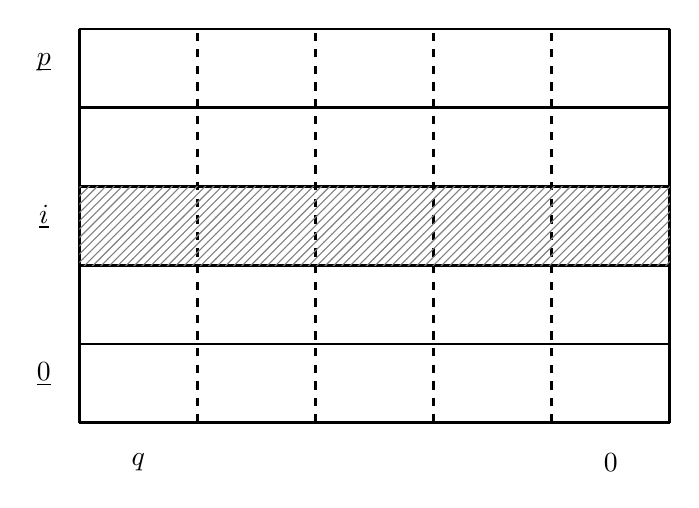
\begin{tikzpicture}[yscale=.8, xscale=1.2, x=1.25cm, y=1.25cm, line width=1pt]
    % Linien.
    \foreach \i in {0,...,5}
    {
        \draw[color=black] (0,\i) -- (5,\i);
    }
    \draw[color=black] (0,0) -- (0,5);
    \draw[color=black] (5,0) -- (5,5);
    \foreach \i in {1,...,4}
    {
        \draw[color=black, dashed] (\i,0) -- (\i,5);
    }
    
    % Beschriftung.
    \draw node at (-.3,4.5) {$\ul p$};
    \draw node at (-.3,2.5) {$\ul i$};
    \draw node at (-.3,0.5) {$\ul 0$};
    
    \draw node at (0.5,-.5) {$q$};
    \draw node at (4.5,-.5) {$0$};
    
    \fill[pattern=north east lines, pattern color=gray] (0,2) -- (0,3) -- (5,3) -- (5,2) -- cycle;
\end{tikzpicture}
}
\end{minipage}
\end{document}